\chapter{Test ss}
 
    \epigraph{``Begin at the beginning," the King said gravely, ``and go on till you come to the end: then stop."}{--- \textup{Lewis Carroll}, Alice in Wonderland}
%     \minitoc
%     \section{test}

    The genomes of chimpanzees and humans are 99.9\% identical, yet the differences between the two species are vast. The relatively few differences in genetic endowment must explain \marginpar[right]{dsdsdsdsd}the possession of language by humans, the extraordinary athleticism of chimpanzees, and myriad other differences. Genomic comparison is allowing researchers to identify candidate genes linked to divergences in the developmental programs of humans and the other primates
%     % \marginnote{%
%     % \centering
%     % \begin{tabular}{lll}
%     % \toprule
%     % 1 & 1 & 1\\
%     % \midrule
%     % 1 & 1 & 0.562 \\
%     % 2 & 1 & 0.910 \\
%     % 3 & 11 & 0.296 \\
%     % \bottomrule
%     % \end{tabular}
%     % \captionof{table}{Sophisticated margin table}
%     % } 
%     and to the emergence of complex functions such as language. The picture will become clearer only as more primate genomes become available for comparison with the human genome.



    \section{sdadsad}
    sdasadsadadsdsadsasd sdaasd
    \lipsum[1-3]
    \subsection{dsadsad}
    dsadasds
    \lipsum[1-4]
    \section{dsad}
    \lipsum[2-6]

%     % \begin{figure}[b]
%     %     \inneralign{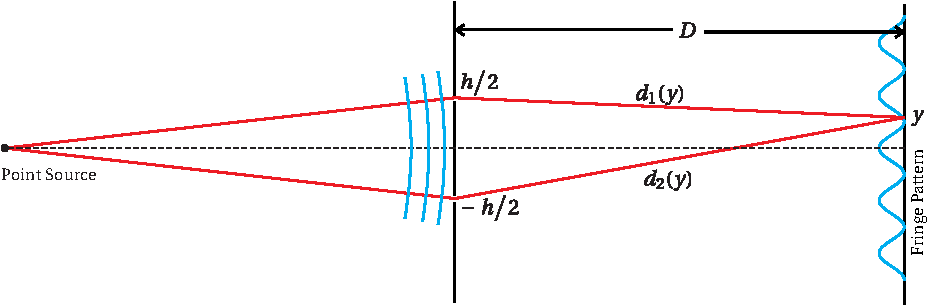
\includegraphics{f08Young}}
%     %     \caption{A point source produces coherent
%     %     (locked phases) light.  When this light which traverses two
%     %    slits and arrives at a screen it produces a fringe pattern.
%     %     }
%     % \end{figure}
    
% \begin{definition}[ds]
%     \begin{equation}
%         \begin{aligned}
%             \mathcal{L} _{\rm{BCE}}(\boldsymbol{\hat{y} },\boldsymbol{y})&=\sum ^N_{i=1}-y^{(i)}\log (\hat{y}^{(i)})- (1-y^{(i)})\log (1-\hat{y}^{(i)})\\
%             &=\sum^N_{i=1}
%             \begin{cases}
%             -\log (\hat{y}^{(i)}),  & \text{for $y^{(i)}=1$} \\
%             -\log (1-\hat{y}^{(i)}), & \text{for $y^{(i)}=0$}
%             \end{cases}
%         \end{aligned}
%     \end{equation}
% \end{definition}


% \lipsum[2]
% \begin{theorem}[ad]
%     abs
% \end{theorem}

% assured
% \begin{lemma}[asd]
%     sdsd
% \end{lemma}


% \lipsum[1]
% \begin{postulate}
%     dsadsa
% \end{postulate}
% \lipsum[4]
% \begin{proof}
%     dsad
% \end{proof}
% \lipsum[4-6]

% % \begin{remark}
% %     borderline west
% % \end{remark}

% \begin{examplebox}{}
%     I use my ``examplebox'' as usual text and margin figure work as they should be but I want my example box spread out to the right margin on an odd page, breakable, and spread out to the left margin on the even page.
%     \tcblower
%     I use my ``examplebox'' as usual text and margin figure work as they should be but I want my example box spread out to the right margin on an odd page, breakable, and spread out to the left margin on the even page.
%   \end{examplebox}

% \lipsum[2-5]
% \begin{corollary}
%     sadsd
% \end{corollary}
% \lipsum[3]
% \begin{proposition}[dsaf]
%     dsadasd
% \end{proposition}

% \begin{tbox}{some extra box}
%     dsadasd
%     Similarly, the differences in genetic endowment among humans are vanishingly small compared with the differences between humans and chimpanzees, yet these differences account for human\citep{li2022limb} variety—including differences in health and in susceptibility to chronic diseases. We have much to learn about the variability in genomic sequence among humans, and the availability of genomic information will almost certainly transform medical diagnosis and treatment. Several monumental studies in which the entire
% \end{tbox}


% A listings example:
% \begin{lstlisting}[language=Python, caption=Python example]
%     import numpy as np

%     def incmatrix(genl1,genl2):
%         m = len(genl1)
%         n = len(genl2)
%         M = None #to become the incidence matrix
%         VT = np.zeros((n*m,1), int)  #dummy variable
        
%         #compute the bitwise xor matrix
%         M1 = bitxormatrix(genl1)
%         M2 = np.triu(bitxormatrix(genl2),1) 
    
%         for i in range(m-1):
%             for j in range(i+1, m):
%                 [r,c] = np.where(M2 == M1[i,j])
%                 for k in range(len(r)):
%                     VT[(i)*n + r[k]] = 1;
%                     VT[(i)*n + c[k]] = 1;
%                     VT[(j)*n + r[k]] = 1;
%                     VT[(j)*n + c[k]] = 1;
                    
%                     if M is None:
%                         M = np.copy(VT)
%                     else:
%                         M = np.concatenate((M, VT), 1)
                    
%                     VT = np.zeros((n*m,1), int)
        
%         return M
%     \end{lstlisting}
% \bibliography{reference}